\chapter{Network Monitoring and Diagnostic}
\label{chapter:monitoring}
We have presented so for explicit mechanisms and techniques to provide
reliability to WR Network. It tolerates (to some extend) component failures and
data corruption. Although, these are the best mechanisms to guarantee continuity
of the message delivery, Network Monitoring and Diagnostic can provide early
detection of future malfunction decreasing the number of failures.
A White Rabbit network provides special features, i.e. precise time
synchronization, deterministic traffic and high reliability of package
delivery, which needs to be carefully monitored. Of course, common parameters 
for standard Ethernet networks, are also important to monitor in order to
obtain full picture of the WR Network performance. This chapter describes the
Monitoring and Diagnostic strategies used in WR Network.


\section{WR-specific Diagnostics}

White Rabbit Network is designed to achieve very demanding requirements in terms
of reliability and determinism of Critical Data Delivery. In such network it is
vital that:
\begin{itemize}
	\item network failure (i.e. not meeting the requirements) can be
precisely diagnosed so that the cause of failure can be immediately fixed,
	\item any suspicious behaviour of the network which might create
potential problem can be early detected and precisely targeted.
\end{itemize}
Therefore, it is important to monitor the WR-specific network characteristics. 
In particular, it is important to know
precise performance of:
\begin{itemize}
	\item \textbf{Timing Data distribution}: UTC clock stability (WR
	      PTP), frequency distribution (SyncE),
	\item \textbf{Control Information distribution} - (\HP Packages and
	      Control Messages lost , \HighPriority),
\end{itemize}


\subsection{Timing Data Distribution Monitoring}

As defined in the IEEE 802.3 \cite{IEEE8023} standard, loosing of three
consecutive symbols on an uplink is interpreted as link-down. It is also
possible to compare phase retrieved from all uplinks and detect instability of
retrieved frequency on an uplink, in such case the stable uplink will be chosen.
This means that monitoring of frequency distribution is limited to  indicate
whether recovery of frequency is working on a given uplink, or not. 


WR PTP offers much more useful parameters regarding the performance than the IEEE 1588
standard \cite{IEEE1588}, which defines the following performance monitoring features:
\begin{itemize}
    \item status,
    \item observed parent offset variance,
    \item observed parent clock phase change rate,
\end{itemize}

White Rabbit will add:
\begin{itemize}
    \item link asymmetry,
    \item port type (uplink/downlink) and mode (WR or non-WR mode)
    \item Rx/Tx delay,
    \item link length,
    \item observed delays variance,
\end{itemize}


\subsection{Control Data Distribution Monitoring}
\label{chap:CTRLdataMonitoring}
The reception of each Control Message by all the WR Receiving Nodes is crucial
for WR Network. Therefore, Data Master shall provide each \ControlMessage\ with
unique ID
number. This enables the Receiving Nodes to identify the fact that
\ControlMessage\ has not been delivered. 


Each \ControlMessage\ is FEC-encoded into a number of \HP\ Packages. FEC allows
to retrieve \ControlMessage\ even if one of the \HP\ Packages is lost. However,
the fact that \HP\ Package was lost might indicate malfunctioning of a component
of the network and upcoming more sever problems. This is why, the FEC encoder
shall provide ot each \HP\ Package with an unique ID number. This ID number shall
consist of:
\begin{itemize}
    \item \ControlMessage\ ID,
    \item ID of \HP\ Package unique within a single \ControlMessage.
\end{itemize}

The redundancy of \ControlMessage\ ID is intentional. It shall be in the
\ControlMessage\ header and \HP\ package header (added by FEC) as the Figure
~\ref{fig:fec_header} shows. It allows to precisely measure delay of a \HP\
packages and easily calculate the delay of a \ControlMessage\ in different
points of the network (a timestamp of sending the first \HP\ minus a timestamp
of receiving the last \HP). 

Each WR Switch shall verify the \HP\ Packages' ID sequence and identify any
unusual behaviour, i.e.:
\begin{itemize}
    \item lost packages,
    \item wrong ID sequence.
\end{itemize}
If a fault is detected by a WR Switch, the Management Node shall
be notify. This enables to precisely locate the cause of a problem, e.g.:
malfunctioning port or link.

As a consequence the following functionalities shall be provided by WR Network:
\begin{itemize}
    \item A WR Management Node shall be able to gather information about
	  timestams of a given \ControlMessage\ (represented by ID) from all the
	  switches and nodes. Such monitoring might be conducted on-demand
	  or/and periodically (polling). 
    \item A WR Management Node shall be notified by WR Switch/Node if a \HP\
	  Package or \ControlMessage\ sequence error is detected.
\end{itemize}


\begin{center}
	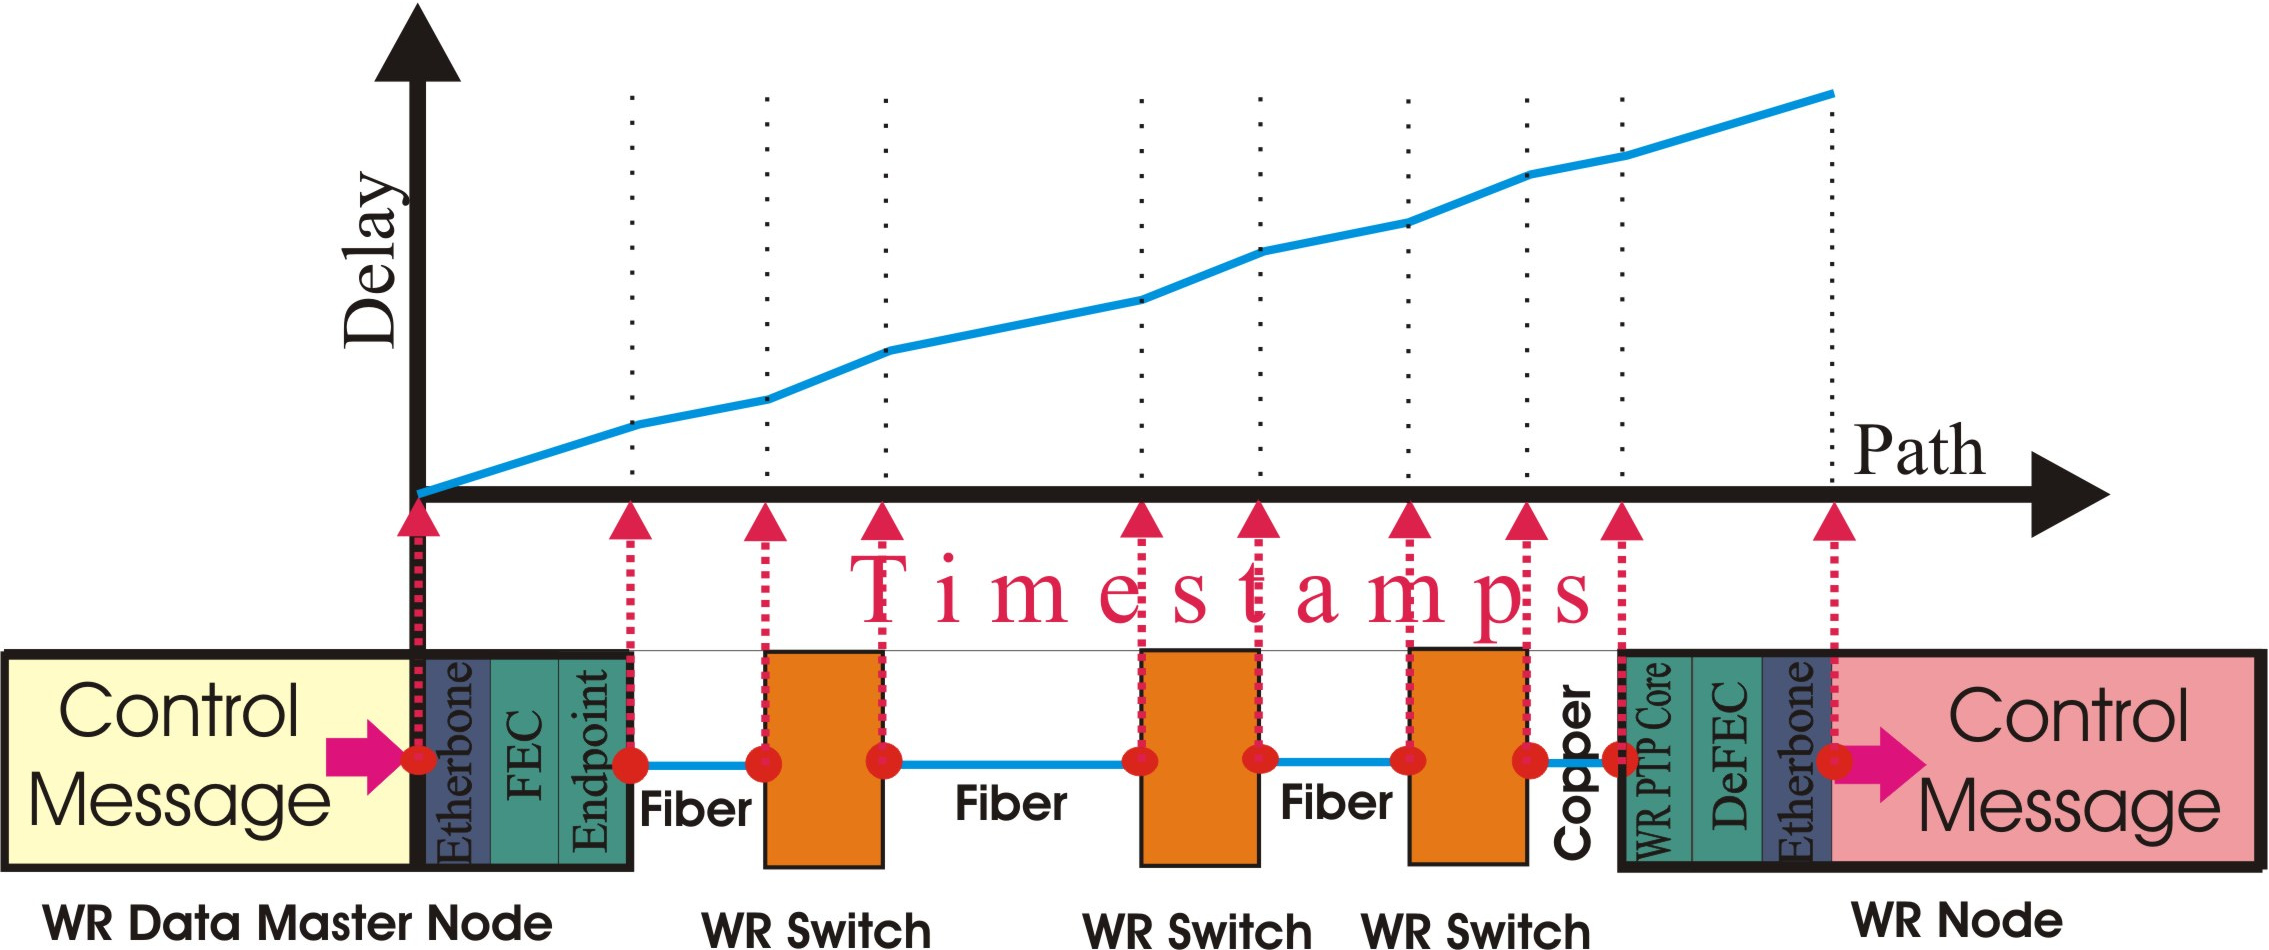
\includegraphics[scale=0.35]{robustness/delayMonitoring.ps}
	\captionof{figure}{\ControlMessage and \HP Package delivery delay
monitoring.}
	\label{fig:pathDelayMonitoring}
\end{center}
 
%%%%%%%%%%%%%%%%%%%%%%%%%%%%%%%%%%%%%%%%%%%%%%%%%%%%%%%%%%%%%%%%%%%%%%%%%%

\section{Flow Monitoring}

Flow monitoring is a scalable technique for measuring network traffic,
collecting, storing, and analysing traffic data. As explained in
Chapter~\ref{chapter:cos}, traffic with different priorities and functionalities
will flow within the White Rabbit Network. Therefore it's of vital importance to
detect diagnose and fix network problems, specially for the \HighPriority\
Traffic \cite{FlowControllers}.

Monitoring traffic flows on the interfaces of the WR Switches
provides visibility, which replaces guesswork of how the network is performing
and provides: 

\begin{itemize}
	\item \textbf{Troubleshooting} Network problems are often first
detectable in abnormal traffic, a flow monitor makes these abnormal traffic
patterns visible to enable rapid identification, diagnosis, and correction.

	\item \textbf{Controlling Congestion} By monitoring the traffic in the 
ports, congested links can be identified and communicated to the Congestion
Control.

	\item \textbf{Routing Profiling} A traffic profile of a network can 
help to understand the bottlenecks and hotspots in the network. 

\end{itemize}

\vspace{10 mm}

A Flow Monitor is based on packet counters with a statistical sampling of the
state of traffic. The sampled information in the switches is immediately sent to
a central collector for analysis. Either the WR Nodes or the Switches will be
endowed with the sFlow Monitor. In the Appendix~\ref{appSFlow} we present the
main characteristics of the monitor.

The sFlow will measure the following parameters of the traffic between
network devices,

\noindent Per-Link:
		\begin{itemize}	
			\item number of packet,
			\item bytes,
			\item packet discarded,
			\item flow or burst of packets,
			\item packets per flow.
		\end{itemize}

\noindent It will also perform End-to-End Measurements of:
		\begin{itemize}	
			\item path delay  
			\item ....
			\item ....
		\end{itemize} 

\noindent The combination of both measurements provides a global picture of the
network.


\vspace{10 mm}

\noindent sFlow shall performance:

\begin{itemize}
	\item Active Measurement - injection of network traffic and study the
reaction to the traffic,
	\item Passive Measurement -  Monitor of the traffic for measurement.
\end{itemize}

\vspace{10 mm}

\noindent The sFlow will configured to achieve:
\begin{itemize}

	\item Reaction Time of ... 
	\item Sampling...
	
\end{itemize}




%%%%%%%%%%%%%%%%%%%%%%%%%%%%%%%%%%%%%%%%%%%%%%%%%%%%%%%%%%%%%%%%%%%%%%%%%%%%%%%%
\subsection{Architecture}


The Figure ~\ref{fig:archi} shows how sFlow, the Flow Control Policy and the
Congestion Control works in every device of a WR network.

The Management Node houses the the sFlow Collector and the DDBB where it will
store the statistic gathered. The Flow Control Policy will be defined and
distributed from this node as well. And as another networking device, the node
is endowed with the Congestion Control mechanism.

As explained, the sFlow agent will monitor the traffic in the switch and will
propagate this statistics to the MMN, but it will also watch over the Flow
Control Policy. In case the sFlow reports a traffic that doesn't respect the
policy the Congestion Control mechanism define for the Critical Broadcast and
the Non-Critical will carry on the actions explained in this chapter.

\begin{center}

        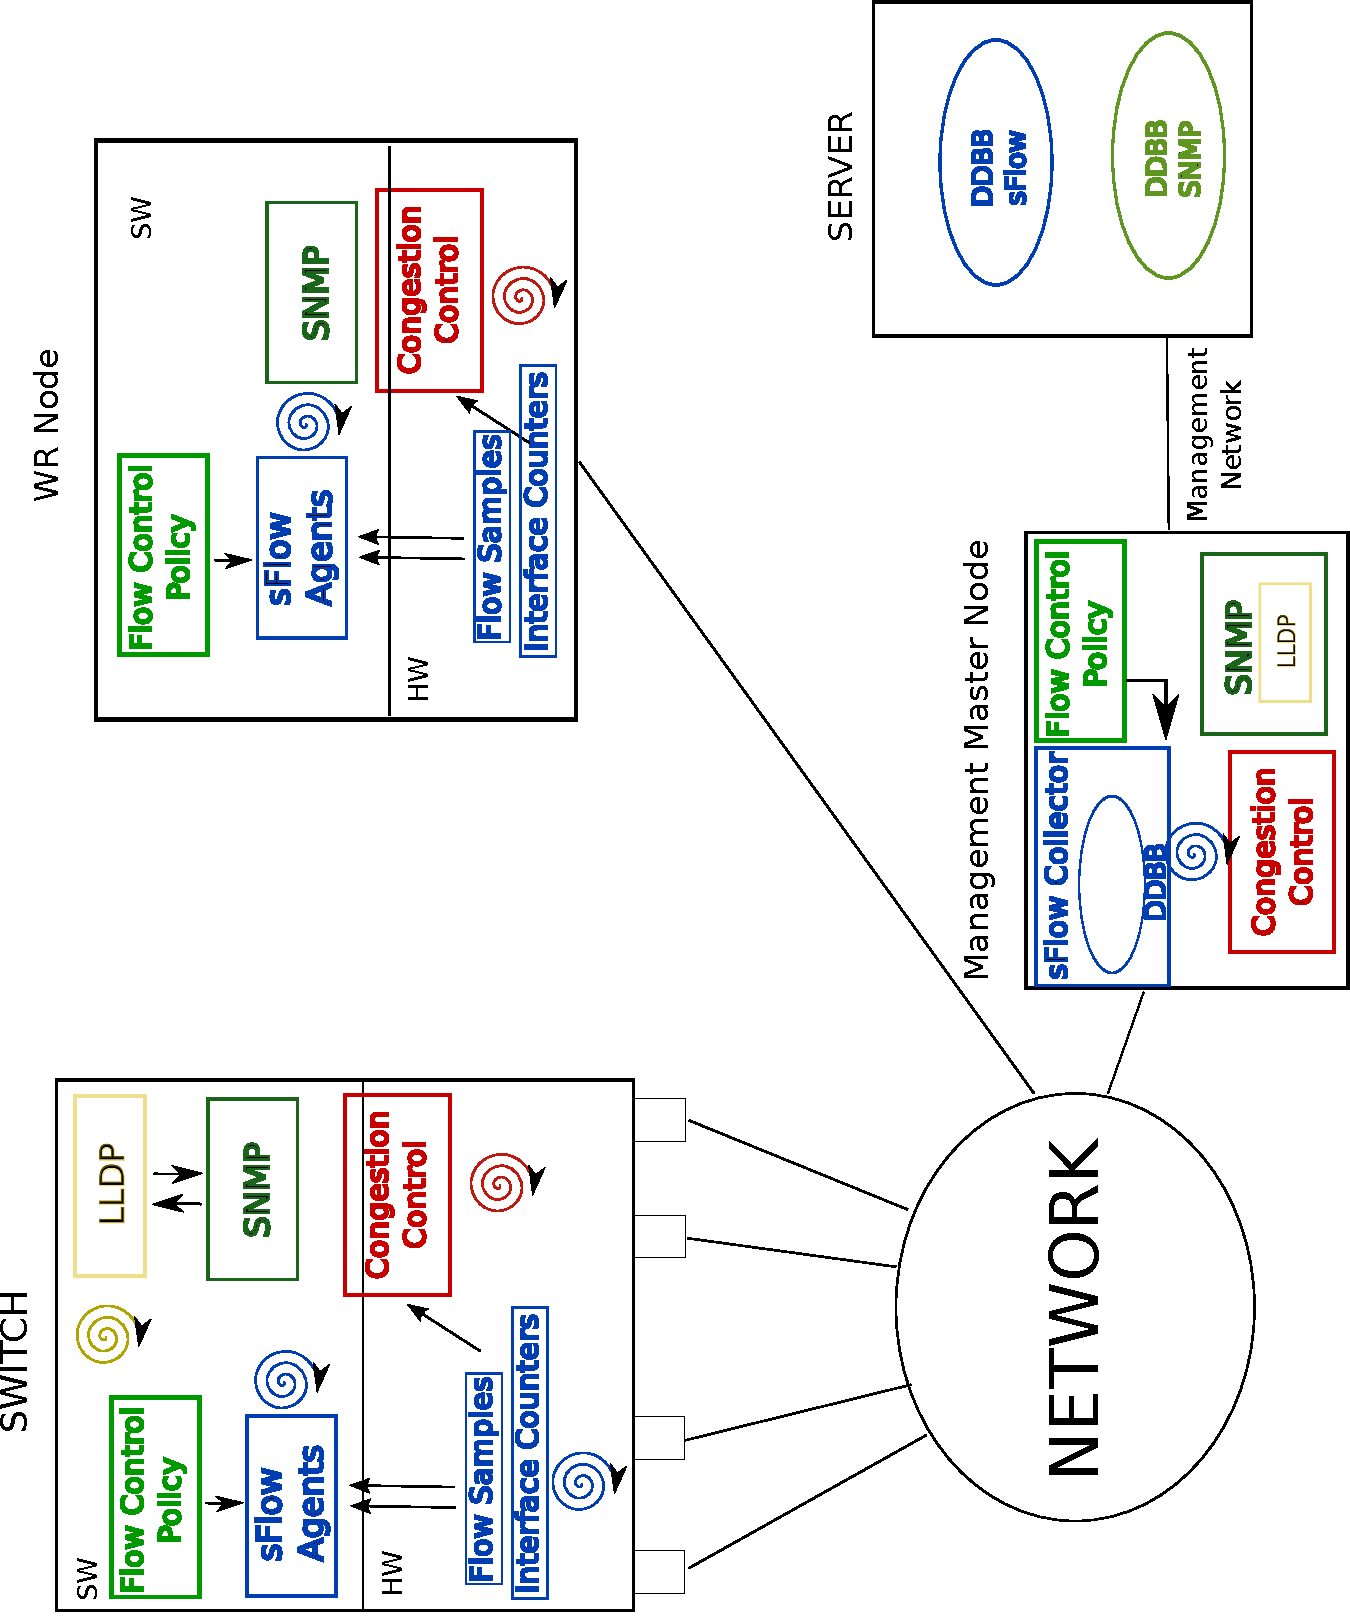
\includegraphics[scale=0.60
]{robustness/architecture_management_flow_congestion_control.ps}
        \captionof{figure}{Architecture of Flow Monitoring, Congestion and Flow
Control}
		\label{fig:archi}
\end{center}

%%%%%%%%%%%%%%%%%%%%%%%%%%%%%%%%%%%%%%%%%%%%%%%%%%%%%%%%%%%%%%%%%%%%%%%%%%%%%%%%
%%%%%%%%%%%%%%%%%%%%%%%%%%%%%%%%%%%%%%%%%%%%%%%%%%%%%%%%%%%%%%%%%%%%%%%%%%%%%%%%



